\begin{frame}{Two Edges}

\begin{columns}[T,onlytextwidth]
    
	\begin{column}{0.5\textwidth}
        \vspace{5.9em}
		\centering
        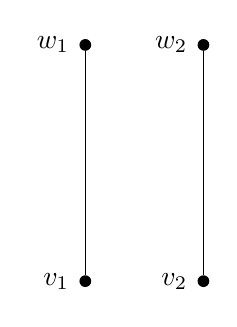
\begin{tikzpicture}[scale=3]
            \node[circle, fill, inner sep=1.5pt, label=left:\(v_1\)] (v1) at (0,0) {};
            \node[circle, fill, inner sep=1.5pt, label=left:\(w_1\)] (w1) at (0,1) {};
            \draw (v1) -- (w1);

            \node[circle, fill, inner sep=1.5pt, label=left:\(v_2\)] (v2) at (0.5,0) {};
            \node[circle, fill, inner sep=1.5pt, label=left:\(w_2\)] (w2) at (0.5,1) {};
            \draw (v2) -- (w2);


        \end{tikzpicture}
        
        \vspace{1em}
		\scriptsize \(\Gamma\) is two disjoint edges
	\end{column}

	\begin{column}{0.5\textwidth}
		\centering
        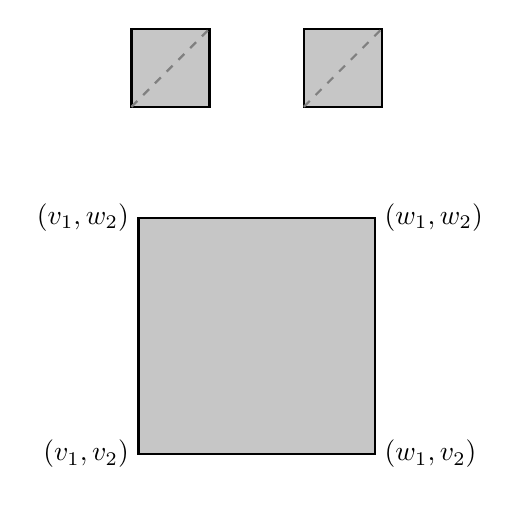
\begin{tikzpicture}[scale=3]

            \fill[gray, opacity=0.45] (0,-.3) rectangle (1,.7);
            \draw[thick] (0,-.3) rectangle (1,.7);
            \node[left] (v1v1) at (0,-.3) {\((v_1, v_2)\)};
            \node[right] (w1w1) at (1,.7) {\((w_1, w_2)\)};
            \node[left] (v1w1) at (0,.7) {\((v_1, w_2)\)};
            \node[right] (w1v1) at (1,-.3) {\((w_1, v_2)\)};


            \fill[gray, opacity=0.45] (-.03,1.5) rectangle (.3, 1.17);
            \draw[thick] (-.03,1.5) rectangle (.3, 1.17);
            \draw[gray, dashed, thick] (-.03,1.17) -- (.3, 1.5);
            %\node[label=above left:{\((v_1,w_1)\)}] (v) at (-.03,1.5) {};
            %\node[label=below right:{\((w_1,v_1)\)}] (w) at (.3,1.17) {};

            \fill[gray, opacity=0.45] (.7,1.5) rectangle (1.03,1.17);
            \draw[thick] (.7,1.5) rectangle (1.03,1.17);
            \draw[gray, dashed, thick] (.7,1.17) -- (1.03,1.5);
            %\node[label=above left:{\((v_2,w_2)\)}] (w) at (.7,1.5) {};
            %\node[label=below right:{\((w_2,v_2)\)}] (w) at (1.03,1.17) {};


        \end{tikzpicture}

        \vspace{1em}
		\scriptsize Part of \(\Conf_2(\Gamma)\).
    \end{column}
\end{columns}

\end{frame}